\documentclass{itatnew}
\usepackage{todonotes}
\usepackage{soul}
\presetkeys{todonotes}{inline}{}
\presetkeys{todonotes}{prepend}{}
\presetkeys{todonotes}{caption=TODO}{}
\def\VH#1{\textcolor{cyan}{VH: \textit{#1}}}
\def\OP#1{\textcolor{purple}{OP: \textit{#1}}}
\def\PB#1{\textcolor{red}{PB: \textit{#1}}}
\def\todo#1{\textcolor{purple}{todo: \textit{#1}}}

\begin{document}

\title{Recurrent Neural Networks for Dialogue State Tracking}

\author{Ondřej Plátek \and Petr Bělohlávek \and Vojtěch Hudeček \and
Josef Válek \and Filip Jurčíček}

\institute{Charles University in Prague,\\
\email{\{oplatek,jurcicek\}@ufal.mff.cuni.cz},\\
\email{me@petrbel.cz},\\
\email{vojta.hudecek@gmail.com},\\
\texttt{http://ufal.mff.cuni.cz/ondrej-platek}}

\maketitle              % typeset the title of the contribution

% \OP{Kde vidite problem se zalamovanim slov} \PB{predict-ing, unreal-istic, individu-ally} vec TeX nechame default


%\OP{Zitra se zeptam na emaily a zda je tam nutne mit webovku. Je povinne udat jednoho korespondencniho autora. Jelikoz z cviceni se do vysledku nedostal ani jeden model udal jsem tam sebe.} \PB{jasne, s tim neni problem, jenom abychom vedeli jak to je :) pripadne by nam mohl ufal udelat mailovky a pak mit adresu ve tvaru \{jeden, druhy, treti, ..\}@ufal.cuni.cz}\\ emaily na ufalu nedostanete - to je takovej porod - jeste vetsi nez ten clanek:)

\begin{abstract}
This paper discuss models for dialogue state tracking using recurrent neural networks (RNN).
We present experiments on standard dialogue state tracking (DST) dataset DSTC2\cite{henderson2014second}.
On one hand, RNN models became state of the art in DST,
on the other hand most state-of-the-art models are only turn-based and require preprocessing specific to evaluated dataset (e.g. DSTC2) in order to achieve state-of-the-art results.
We implemented two architectures which can be used in incremental settings and requires almost no preprocessing.
We compare their performance to the benchmarks on DSTC2 and discuss their properties.
With only a trivial preprocessing performance of our models is close to the state-of-the-art results.
\end{abstract}
%
\section{Introduction}
%
The dialogue state tracking (DST) is a standard and important task for evaluating conversational agents\cite{williams2013dialog, henderson2014second, henderson2014third}.
The dialogue state tracker summarizes hidden information state (HIS)\cite{young2010hidden} of users goal from the conversation history.
Users goals are expressed in a~formal language, typically represented as a dialogue act item (DAI). Dialogue act item is a triple $(actionType, slotName, slotValue)$.
It was shown that with a better dialogue state tracking of HIS the conversation agents achieve better success rate in overall completion of the their task\cite{jurvcivcek2012reinforcement}.
The dialogue state tracking translates ambiguous natural language into the formal language which is convenient for reasoning and accessing external knowledge. Reasoning as well as use of external knowledge are crucial to successful conversation in task oriented dialogue.

Most state-of-the-art system in DST have reported their performance on DSTC2 dataset\cite{henderson2014second}. 
The full dataset is freely available since January 2014 and contains 1612 dialogues in training set, 506 dialogues in development set and 1117 dialogues in the test set.
The conversations are annotated at turn level where the hidden information state was annotated manually in form of $(actionType, slotName, slotValue)$ according to the domain ontology.
The ontology of DSTC2 captures a~restaurant domain and was also manually designed.
In addition, the dataset contains a database of restaurants and their properties\footnote{There are six columns in the database: name, food, price\_range, area, telephone, address.}.

Our experiments predict the dialogue state only ASR transcriptions of the conversation history and a word feature which fires if a word may be a property from the database.
We argue that using only database values instead of full ontology is not only simpler but also more natural because the system can inform users only about the values in the database.
In addition, we show in Section~\ref{sec:eval} that we achieve strong performance.

In our experiments, we focus only on the {\it goal} slot predictions because the other groups are trivial to predict\footnote{The slots {\it Requested} and {\it Method} have accuracies 0.95 and 0.95 on the test set according to state-of-the-art\cite{williams2014web}.} and thus obtaining annotated data for new domain is considerably simpler.
We show that limiting ourselves to {\it goal} slot values, which are not only wanted by the user but which must be also present in the database, we lose only a little accuracy if any.
See Section~\ref{sec:exp} for details.
Tracking only the properties of restaurants in the dialogue state allow us to annotate the dialogue state as a query to the database. Such approach allows us to use much simpler interface for human annotators than selecting many options from DSTC2 ontology.
Simplification of the dialogue state and still achieving high accuracy allows better portability of proposed models to new domains.

We also show that DSTC2 dataset suffers from differences between the train and test data sets.
The DSTC2 test set was collected from different systems\cite{henderson2014second}.
Since the data of training, development and test set are distributed differently, the resulting performance between training and test accuracy is rather high.
% TODO opravime v camera ready verzi \PB{vagni formulace, nechceme reportovat radeji cislo?}. 
Our experiments show that one can obtain better results by splitting the data randomly.
As a result, we conclude that DSTC2 might suggest too pessimistic view of the state-of-the-art methods in dialogue state tracking caused by the data distribution mismatch.

Our contribution is three fold. 
At first, in Section~\ref{sec:model} we compare two different architectures using RNN for dialogue state tracking.
Secondly, in~Section~\ref{sec:eval} we describe state-of-the art word-by-word dialogue state trackers architectures and propose a new encoder-decoder architecture for DST task.
Finally, in~Section~\ref{sec:eval} we show that obtaining excellent results on DSTC2 dataset is very demanding because of the training and test set dissimilarity. In contrast, we obtained much better results just by random resplitting of the DSTC2 data.
% TODO measure significance and report significant improvement

\section{Models}
\label{sec:model}

Our models are all based on Recurrent Neural Network encoder\cite{werbos1990backpropagation}. Similarly to RNN encoder\cite{zilka2015incremental}, the models update their hidden states $h_{enc}$ after processing each word.
The models differ only in the way they predict {\it goal} labels, i.e. $food$, $area$ and $price range$, from the RNN's encoded state.

% The first model predicts the triples of slot values $(food, area, price range)$ jointly from the encoder hidden state $h_{enc}$.
The first model predicts the labels independently by employing three independent classifiers, each predicting either $food$, $area$ or $price range$ based on $h_{enc}$.
The second model uses a decoder in order to predict values one after each other from the $h_{enc}$. It is an implementation of the encoder-decoder model, which has been successfully used in machine translation\cite{bahdanau2014neural}.

The RNN encoders take word embedding and several binary features as the input at each step.
% TODO pridat referenci na word embeddingy
The binary features for each word are the speaker role, representing either user or system, and also indicators describing whether the word is part of some named entity representing a value from the database.
Since DSTC2 database is a simple table with six columns, we introduce six binary features firing if the word is a substring of named entity at given column.
For example, the word {\it indian} will not only trigger the feature for column $food$ and its value {\it indian} but also for column restaurant $name$ and its value {\it indian heaven}.

Both models were implemented using TensorFlow\cite{abaditensorflow} framework. By introducing more and more complex models, we aim to overcome the data sparsity problem and incorrect independence assumptions.

\subsection{Predicting labels jointly}
\label{sec:joint}
Joint model uses a single classifier to predict a tuple of slots (see Figure~\ref{fig:encjoint}).
The model is easy to implement and it optimizes directly the evaluation metric of predicting the labels jointly.
However, with increasing number of slots the model suffers from the curse of dimensionality and therefore it is not convenient for small datasets.
\begin{figure}
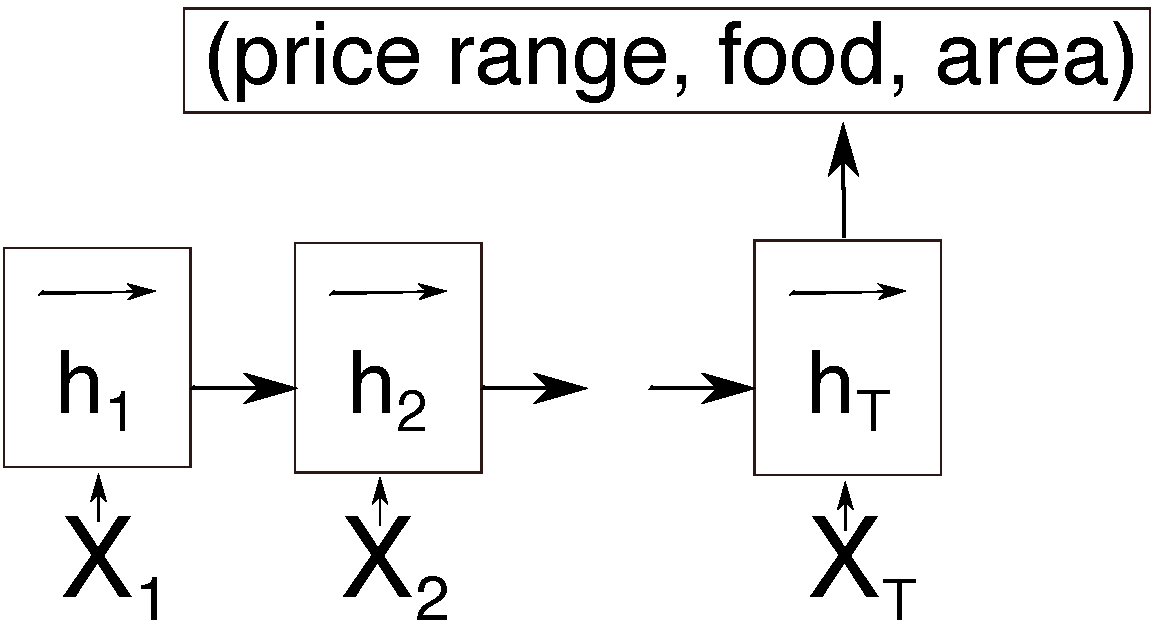
\includegraphics[width=0.5\textwidth]{encoder_joint}
\caption{The joint label predictions using RNN.}
\label{fig:encjoint}
\end{figure}

\subsection{Predicting labels independently}
\label{sec:indep}
Independent slots prediction using one classifier per each slot is also straightforward to implement.
It does not suffer from the curse of dimensionality but it introduce unrealistic assumption of uncorrelated slot properties.
In case of DSTC2 and Cambridge restaurant domain, it is hard to believe that e.g. slots $area$ and $price range$ do not correlate.
% \PB{neni 'hard' moc informal? mozna 'difficult'?}\VH{nebo proste: it's unlikely that..}  ja mam docela rad neformalni vyrazy. Necham to tak. Muzem v camera ready prodiskutovat
\begin{figure}
\includegraphics[width=0.5\textwidth]{encoder}
\caption{The RNN encodes the word history into dialogue state $h_T$ and predicts slot values independently.}
\label{fig:encind}
\end{figure}

\subsection{Encoder decoder framework}
\label{sec:encdec}
The encoder decoder model with attention\cite{bahdanau2014neural} is the most sophisticated model we used for slot predictions.
To our knowledge, we are first who used this model for the task of slot predictions.
The model is typically used in machine translation, since it's  able to handle longer sequences with good accuracy and it captures correlation between the decoded slots easily\cite{bahdanau2014neural}. %\PB{kolik? nebo reference?} -> reference je Bahdanau na konci vety

The disadvantage of this model is its complexity.
Firstly, the model is not trivial to implement\footnote{We modified code from TensorFlow `seq2seq` module.}. Secondly, the decoding time is quadratic in length of the decoded tuples.
However, it is trivial to encode dialogue state tracking as sequence-to-sequence problem. Given the the dialogue history as the input sequence, we trained the model to predict always four labels which represent the first, the second, the third slot and the~end-of-string symbol.
Since our target sequence is always of length four, the model does not suffer from long decoding time. 
%\PB{In contrast, the decoding consumes asymptotically constant time regardless the input.}  to mi prijde zbytecny, to ocekavas.
\begin{figure}
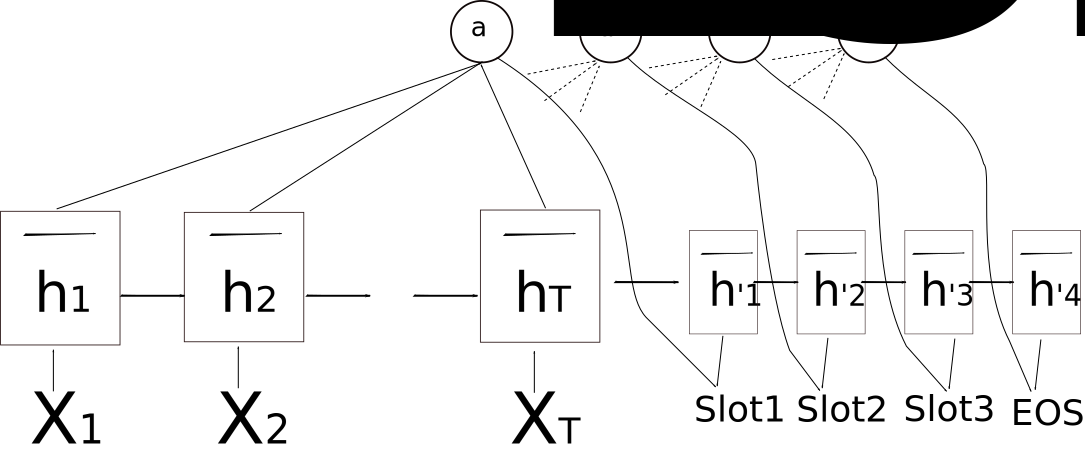
\includegraphics[width=0.5\textwidth]{encdec}
\caption{Encoder decoder with attention predicts goals.}
\label{fig:encdec}
\end{figure}

\section{Experiments}
\label{sec:exp}

% TODO it would be interesting to turn of the additional DB features for the encoder and compare it to L. Zilka's work
We report results on the standard split where we used 516 dialogues as a validation set for early stopping\cite{prechelt1998early} and 90\% for training. The joint slot accuracy is predicted from ASR transcription only.
For the results on the standard split of DSTC2 see see~Table~\ref{tab:dstc}.
We also evaluated the models randomly splitted DSTC2 dataset and the details are described in~Subsection\ref{sec:split}.
Note that we measure accuracy with schedule 2 with using the official evaluation scripts in all our experiments.

% \todo{nechceme reportovat i train a valid? me to vetsinou v clancich zajima} muzem kdyz to stihnem, ale validace na trenovani trva dlouho a nechce se mi to prepocitavat na validacni sade to mame

For all our experiments, we train word embeddings of size 100 and use the encoder state size of size 100\, together with a dropout keep probability of $0.7$ for both encoder inputs and outputs.
These parameters where selected by a grid search on the hyperparameters.

\subsection{Training}
\label{sec:train}
% TODO describe vocabularies and shared embeddings for encoder-decoder
The training is optimized using the cross-entropy loss function and Adam optimizer\cite{kingma2014adam} with batch size ten.
We train predicting goal slot values at the end of each turn by feeding the model by the turn slot labels $labels_t$ and the whole dialogue history until the turn $t$.
Since the dialogue lengths vary a lot\footnote{The maximum turn length is 487 words and 95\% percentile is 205 words on the training set.} and we batch our inputs, we separated the dialogues into ten buckets accordingly to their lengths in order to provide computational speed-up. We reshuffle the data after each epoch only within each bucket.
Early stopping with patience\cite{prechelt1998early} of four models is run after each epoch on validation set.

\subsection{Labels representation evaluation}
\label{sec:eval}
The predicted labels not only depend on the last turn, but on the dialogue full history as well, which makes the task very challenging.
Our informal experiments showed that optimizing the training only on the last turn\footnote{The prediction was conditioned on full history but we back-propagated the error only in words for last turn.} degrades the performance by more than 40\%.

Predicting the labels jointly is quite challenging because the distribution of the labels is skewed as demonstrated in~Figure~\ref{fig:labels}.
As some of the labels combinations are very rare, they occur only in the development and test set so the joint model is not able to predict them.
During first informal experiments the model performed poorly arguably due to data sparsity of slot triples and we do not focus in further evaluation.

\begin{figure}
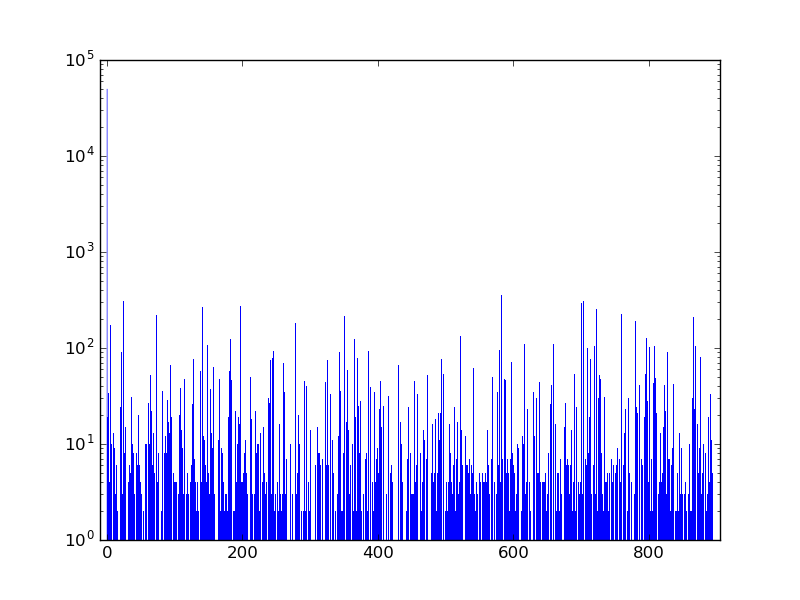
\includegraphics[width=0.5\textwidth]{dstc2_goals_joint_log_scale}
\caption{The log-scaled histogram of joint labels. The x axis represents the id of the $(food, area, pricerange)$ triple.}
\label{fig:labels}
\end{figure}

% The model with independent label prediction obtained much better performance on each slot individually as expected, but also it surprisingly outperformed the joint model in the joint prediction.
% We hypothesize that with larger amount of data the joint model would suffer less from data sparsity and perform better.
% This claim is supported by comparison of joint and independent models performance on the original DSTC2 dataset.
The model with independent label prediction is a strong baseline which was used among others in work of~\cite{zilka2015incremental}.
The model sufferers less from from data mismatch because it does not model correlation between predicted labels.
This property can explain smaller performance dropped between the test set from reshuffled data and the official test set in comparison to encoder-decoder model.
In the official DSTC2 dataset, the training and test set differ much more than on our resplitted version (see Table~\ref{tab:dstc} and Table~\ref{tab:resplit} for details).

\begin{table}
\caption{Accuracy on development and test set}
\begin{center}
\begin{tabular}{r@{\quad}rll}
\hline
\multicolumn{1}{l}{\rule{0pt}{12pt}
                   Model}&\multicolumn{1}{l}{Dev set}&\multicolumn{2}{l}{Test set}\\[2pt]
\hline\rule{0pt}{12pt}
% Joint  &     ?&  todo \\
% /a/SSD/oplatek/e2end/log/2016-06-08-17-31-38.400-dstc-INDEP_labels-d0.7-w100-e100/
% /a/SSD/oplatek/e2end/log/TEST-ORIGINAL-2016-06-08-17-31-38.400dstc-INDEP_labels-d0.7-w100-e100-reward-0.9080-step-0036224
Indep  &   0.91 & 0.76 \\
EncDec &   0.94 & 0.73 \\
\hline
\end{tabular}
\end{center}
\label{tab:dstc}
\end{table}

Since the encoder decoder architecture is much more general, it also needs to learn how to predict only three slot labels in the correct order.
It turned out, that the architecture learned to predict tuples of four with three slot values and the end-of-string (EOS) symbol quickly, even before seeing first half of training data in the first epoch.
% TODO rewrite betteh than\VH{..before the first half of training data was presented/introduced to it}.
At the end of first epoch it made no more mistakes on predicting slot values in the incorrect order.
The encoder decoder strongly outperformed the previous models and the time needed for learning the output structure was surprisingly short .\footnote{The best model weights were found after 18 to 23 epochs for all model architectures.}
% TODO jak dlouho trvala epocha

\subsection{Data preparation experiments}
\label{sec:split}
The data for DSTC2 test set were obtained from another system than the data for validation and training set.\cite{henderson2014second}.
We wanted to investigate how this influences the complexity of the dataset so we merged all DSTC2 data together and created splits of 80\%, 10\% and 10\% for training, development and test set.
The results in Table~\ref{tab:resplit} show that the complexity of the task dropped significantly.

\begin{table}
\caption{Accuracy on resplitted DSTC2 development and test set.}
\begin{center}
\begin{tabular}{r@{\quad}rll}
\hline
\multicolumn{1}{l}{\rule{0pt}{12pt}
                   Model}&\multicolumn{1}{l}{Dev set}&\multicolumn{2}{l}{Test set}\\[2pt]
\hline\rule{0pt}{12pt}
% Joint  &     ?&  todo \\
Indep  &   0.87 & 0.89 \\
EncDec &   0.94 & 0.91 \\
\hline
\end{tabular}
\end{center}
\label{tab:resplit}
\end{table}

\section{Related work}
\label{sec:related}
% NEJDE musime se drzet sablony - ano je trochu nesikovna\todo{full-name reference, nejde pouzit citet ani citep, proc?}
Our system is related to RNN tracker of \cite{zilka2015incremental}
which reported near state-of-the art results on DSTC2 dataset and was the first incremental system which was able to update the dialogue state word-by-word with such accuracy.
In contrast to work of \cite{zilka2015incremental}, we use no abstraction of slot values. Instead, we add the additional features as described in Section~\ref{sec:model}.
The first system which used Neural Network for dialogue state tracking \cite{henderson2013deep} used feed forward network and manually engineered more than ten features across different levels of abstraction of the user input, including spoken language understanding component (SLU).
In our work, we focus on simplifying the architecture, hence we used only features which were explicitly given by the dialogue history word representation and the database.

The system of \cite{henderson2014word} gives state-of-the-art results and, similarly to our system, it predicts the dialogue state from words by employing a recurrent neural networks.
On the other hand, Henderson's et al system heavily relies on the user input abstraction.
Another dialogue state tracker with LSTM was used in reinforcement setting but the authors also used information from SLU pipeline.\cite{lee2016dialog}

It is worth noting that there are first attempts to train end-to-end dialogue system even without explicitly modeling dialogue state\cite{bordes2016learning} which further simplifies the architecture of a dialogue system.
However, the reported end-to-end model was evaluated only on artificial dataset and cannot be compared to DSTC2 dataset directly.
An interesting approach present work\cite{vodolan2015hybrid} which that combines a rule based and a machine learning based approach to belief state tracking.
Their work clearly identifies the handcrafted features which can be easily modified. The features are fed to LSTM which performs a dialog-state update.
The system is the best performing system on live SLU input which is the main difference to our setup which uses only live ASR transcriptions.

\section{Conclusion}
\label{sec:conc}

We presented two dialogue state tracking models which represent the state-of-the-art architectures using recurrent neural networks and compared them with each other.
To our knowledge, we are the first who used encoder-decoder model for the dialogue state tracking task, and we encourage others to do so, because it outperformed other standard RNN models.
We also observed that obtaining high accuracy for dialogue state tracking on DSTC2 test set is notoriously hard and that the task become substantially easier if the data is reshuffled.

The code is published under permissive Apache license at Github \url{https://github.com/oplatek/e2end/}. \footnote{Some informal experiments were conducted using during summer semester of the Statistical Dialogue System class and can be also found on Github: https://github.com/oplatek/sds-tracker}
\subsection*{Future work}
Among our first next steps will be im
We also plan to predict all slots tracked in the DSTC2 dataset.
Another direction of our future work will focus on collecting and annotating more data which would allow us to evaluate the models on another task-oriented dataset.

\subsection*{Acknowledgment}
We would like to thank Mirek Vodolán for help with evaluation scripts.
This research was partly funded by the Ministry of Education, Youth and Sports of the Czech Republic under the grant agreement LK11221, core research funding, grant GAUK 1915/2015, and also partially supported by SVV project number 260 224. 
We gratefully acknowledge the support of NVIDIA Corporation with the donation of the Tesla K40c GPU used for this research.
Cloud computational resources were provided by the MetaCentrum under the program LM2010005 and the CERIT-SC under the program Centre CERIT Scientific Cloud, part of the Operational Program Research and Development for Innovations, Reg. no. CZ.1.05/3.2.00/08.0144.
% TODO myslim, ze to mam dobre, ale v camera ready to zkontrolujem - nestiham. \PB{nemusi byt podekovani metacentru v nejake jejich oficialni podobe - link v komentari?} %https://wiki.metacentrum.cz/wiki/Pravidla_vyu%C5%BEit%C3%AD_MetaVO/Pod%C4%9Bkov%C3%A1n%C3%AD

\bibliographystyle{plain}
\bibliography{samplearticle}
\end{document}
